\chapter{Implementáció} \label{implementationChapter}

Vegyük górcső alá a témában végzett programozói munkámat. Összesen 4 algoritmussal foglalkoztam, amiket logikailag egymásra építve kezeltem:
TSP  \(\rightarrow\) VRP \(\rightarrow\) CVRP \(\rightarrow\) (C)VRPTW

\section{Hangyakolónia algoritmus}
A munkám során a felsorolt algoritmusok mindegyikét a hangyakolónia optimalizációval oldottam meg.

\subsection{Adatstruktúrák}
Az útvonaltervezési problémák gráfokon futnak, ezért elsődleges feladatom annak eldöntése volt, hogy milyen formában tároljam a gráfokat. Egyik legalapvetőbb megadási mód a szomszédossági mátrixával történő reprezentáció. Ennek előnye, hogy az egyes csúcsokhoz tartozó élek könnyen, direkt lekérdezhetőek, ezért a rajtuk végzett műveletek gyorsabbak lehetnek. Hátránya azonban, hogy minél kevesebb él van a gráfban, annál pazarlóbbá válik ez a megadás. Később tekintünk egyéb megadási módokat is, de most azokkal nem foglalkozok.
Az adattípusok megválasztásában eltérőek az egyes megvalósítások: az első TSP verzióban például minden lebegőpontos számot \textit{double} típusú változóban tárolok, míg a többi algoritmusnál \textit{float} adatípust alkalmazok. A váltás hátterében az áll, hogy kipróbálva az első algoritmust azt tapasztaltam, hogy nem javít érdemben a valószínűségek dupla pontosságú számítása, cserébe sokat lehet spórolni a futásidőn egyszeres pontossággal.


\subsection{Feromonok nyilvántartása}
A feromonokat az élekhez rendelem, ezért egy, az eredeti gráf topológiájával megegyező, teljes gráfban tárolom. A gráfélek eltárolása már másképpen történhet. 

\subsubsection{TSP}
A TSP során egy NxN-es mátrix által adott feromongráfon egyértelműen végrehajtható mohó algoritmus, vagyis olyan döntéshozatal-sorozat, hogy minden csúcsból abba a következő pontba megyünk, ahova a legtöbb feromon vezet (kivéve ha az a kezdőcsúcsba vezet, és még maradtak bejáratlan csúcsok). Hogy megtartsam az implementáció egyszerűségét, a TSP során tényleg NxN-es 2 dimenziós mátrixban tárolom a feromonértékeket. Tehát a TSP feromonmátrix a kezdőpillanatban a következő:

$\begin{pmatrix}
	0 & P_{0,1} & P_{0,2} & \cdots & P_{0,n-1}\\ 
	P_{1,0} & 0 & P_{1,2} & \cdots & P_{1,n-1} \\
	\vdots & & \ddots \\
	P_{n-1,0} & P_{n-1,1} & P_{n-1,2} & \cdots & 0
\end{pmatrix}$

Ahol P{\scriptsize i,j} az i-ből j-be él kezdeti feromonértéke. \( \forall i\in V(G) : P_{i,i}=0 \), mert a gráfunk egyszerű, nincs benne hurokél. Praktikusan \( P_{i,j}=0 \) ha az input gráfban \(v_{i,j}\) nincs behúzva. Ekkor már az első próbálkozások sem próbálnak meg arra menni. Ez a kikötés nem kötelező, előbb-utóbb ezen éleket úgyis elhalnának a feromonok. 

\subsubsection{VRP variánsok}
A VRP esetében kicsit bonyolultabb a helyzet. Ha felírjuk egymás után az egyes járművek bejárási sorrendjét azt láthatjuk, hogy olyan, mintha több TSP-t hajtottunk volna végre egymás után. Képzeletben majdnem ez is történt. Úgy álltam hozzá a több útvonalhoz, hogy fejben kifeszítettem őket egy nagy körré. A kezdőcsúcs helyére gondolhatjuk azt, hogy k db csúcs van ott, akik egymástól 0 távolságra vannak. A gondolatmenetemet a \ref{tsp-to-vrp}. ábrán illusztrálom. 

\begin{figure}[ht!]
	\centering
	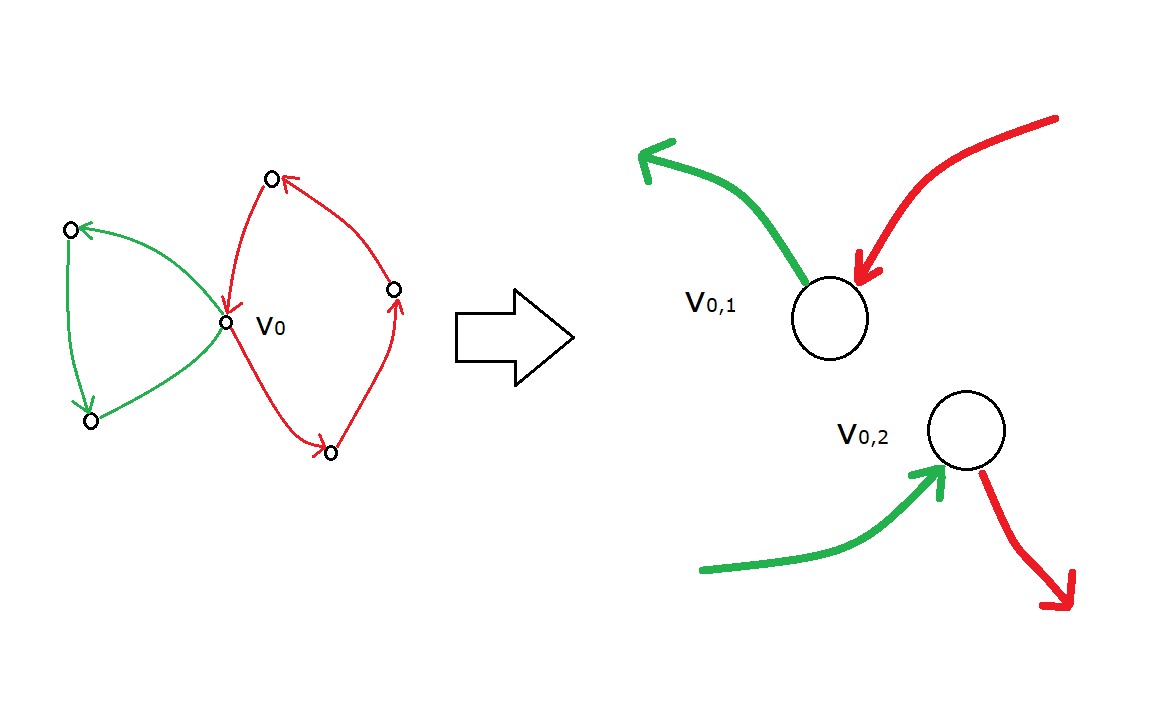
\includegraphics[width=0.5\textwidth]{figures/tsp-to-vrp.png}
	\caption{A VRP visszavezethető a TSP-re, ha az egyes utakat képzeletben összefűzzük egy nagy körré \label{tsp-to-vrp} }
\end{figure}

Egy n csúcsot k járművel bejáró VRP visszavezethető egy n+k-1 csúcsú TSP-re. Az, hogy milyen egyéb feltételeket tűzünk még ki a feladatba, a feromonok nyilvántartásának módját nem befolyásolja, csak ott módosít, hogy hiába vezet út az adott körön, ha például a járművel kapacitásfeltétele sérül. Olyankor egyáltalán nem veszem figyelembe az adott megoldást.

\textcolor{red}{BEFEJEZETLEN SZÖVEGRÉSZ}
%TODO folytani

\subsection{A rulettkerék algoritmus }
Az algoritmusaimban többször feltűnik a random számok kezelése. Hallgatótársam, Tóth Andor Márk sokat foglalkozott a témával, és diplomamunkájából sokat tanulhattam a témában \cite{alg_optim}. Valószínűségszámításból tudjuk, hogy igazi véletlen számok nem léteznek. Elméletileg nincs is semmi értelme ennek a fogalomnak. Nézzük például a klasszikus példát: a pénzérme feldobását, ami a földre érve fejjel vagy írással felfelé landol (vagy egyes nagy sikerű filmekben a sirály még a földet érés előtt elkapja és elviszi). Ha a tér minden egyes pontjában pontosan ismernénk a különböző légnyomásértékeket, valamint tökéletesen tisztában lennénk a feldobás dinamikai jellemzőivel, mindig pontosan tudnánk, hogy melyik oldalára fog esni az érme. A véletlen illúzióját ezen ismeretek hiánya okozza. Póker közben is feltehetően nem ismerjük a keverő pontos technikáját, ezért az osztott lapok jó esetben véletlenszerűnek hatnak. A számítógépek alapesetben determinisztikus gépek, hiszen adott utasításokat hajtanak végre. 
A CUDA is úgynevezett pszeudorandomszám-generátor elvét követi. Ez tökéletesen meghatározható egy kezdeti érték alapján, kell egy seed, ami viszont már független lehet a számítógéptől. Én a klasszikus megoldást választottam, miszerint az 1970. január 1. éjfél óta eltelt másodpercek számát vettem seednek.
GPU oldalon a CuRand függvénykönyvtár videokártyás támogatást biztosít pszeudorandom számok generálására, ehhez a következő egyszerű kernelt kell futtatni:

\begin{lstlisting}[style=CStyle]
	// Initializes a random seed for each different threads
	__global__ void setup_kernel(curandState* state, unsigned long seed)
	{
		int id = blockIdx.x * blockDim.x + threadIdx.x;
		curand_init(seed, id, id, &state[id]);
	}
\end{lstlisting}

A kernelt CPU oldalról kell felhívni a kiválasztott seeddel.

\begin{lstlisting}[style=CStyle]
	srand(time(0)); // Need seeds for random solutions
	
	...
	
	setup_kernel <<< BlockNum, threadPerBlock >>> (d_kernelParams.state, time(NULL) * rand());
\end{lstlisting}

\begin{lstlisting}[style=CStyle]
	
\end{lstlisting}


\section{TSP első verzió} \label{TSP_v1_SubSection}
Korábban már volt róla szó, de az útvonatkeresési algoritmusok ezen családjának legegyszerűbb tagja a TSP, ezért ezzel érdemes kezdenie annak, aki szeretne elmélyülni a problémakörben. Én is így tettem. Amikor még az Önálló laboratóriumi munkám során megismertem a genetikus algoritmusokat, az első feladatom a TSP megvalósítása volt CUDA nyelven. Azért tartom fontosnak kiemelni a TSP programom első verzióját, mert elsőkörben teljesen rendszertelenül álltam a problémához, nem tekintettem a feladatra egy nagyobb téma részeként. Ez később nehezen bővithető lett volna, ezért a következő verziókat teljesen a nulláról kellett felépítenem.

A mellékletben elérhető a teljes TSP\_v1 kód, jelenleg néhány fontosabb elemet/fogalmat szeretnék kiemelni belőle.
Bevezettem egy globális változót a hangyák (threadek) számának állítására. Jelenleg konstans, amennyiben a felhasználó egyéb számú párhuzamosítást szeretne, sajnos még bele kell nyúljon a forráskódba:

\begin{lstlisting}[style=CStyle]
	// Number of threads = number of ants
	const int ants = 1024;
\end{lstlisting}

Van még néhány olyan algoritmus paraméter, ami a futás során változatlan, viszont értékük befolyásolja a futásidőt, illetve a végeredményt. Kiszerveztem őket makróba, hogy csak egy helyen kelljen változtatni.

\begin{lstlisting}[style=CStyle]
	// Repetition constants
	#define REPETITIONS 10
	#define RANDOM_GENERATIONS 20
	#define FOLLOWER_GENERATIONS 500
	
	// Pheromon matrix constants
	#define RHO 0.75  // Reduction ratio of previous pheromon value
	#define REWARD_MULTIPLIER 100   // Reward multiplier after finding a shortest path until then
	#define INITIAL_PHEROMONE_VALUE 1000    // Initial value of elements in the Pheromone matrix
	
	#define SERIALMAXTRIES 10    // Number of serial processes
\end{lstlisting}

Először a "Repetition" konstansokról: Az algoritmus így működik: Csináld REPETITIONS alkalommal, hogy jön RANDOM\_GENERATIONS iteráció olyan hangya, aki teljesen véletlenszerűen végigmegy a gráfon, majd őket követi FOLLOWER\_GENERATIONS iterációban olyan hangya, aki a feromon alapján dönti el az útját. Minél több iterációt hajtunk végre, annál több utat vizsgálunk meg, és elvileg annál pontosabb lehet a végeredmény.
Az előbbiektől némileg elkülönül a SERIAL\_MAXTRIES, ami azért felel, hogy többször lefuttathassuk egymás után a GPU kernelt. Mivel az ACO egy heurisztikus algoritmus, futásonként más és más eredményt szolgáltat. Éppen ezért érdemes lehet többször (például 10-szer) egymás után végrehajtani az algoritmust, és megvizsgálni az egyes eredményeket. Ilyenkor végső eredménynek célszerű a legrövidebb megoldást venni. Sajnos a tesztelések során azt tapasztaltam, hogy a GPU főleg amikor több szálon dolgozik, mint ami fizikailag elérhető CUDA core formájában, gyakran hibázik, és nem vagy rosszul ír át memóriaterületeket. Azon memóriaterület, mely tárolja azt aktuális minimális szekvenciát, rendkívül ki van téve 

\textcolor{red}{Hardver ismertetése}
\textcolor{red}{Többi algoritmus ismertetése}

%TODO többi algoritmus?



